\section{Il programma}
Per semplicit\`a e allegerire i calcoli ho impostato $\hbar=1$, 
Gli eseguibili compilabili dal Makefile sono i seguenti, nei commenti \`e spiegato come eseguirli:
\lstinputlisting[language=make, firstline = 16, lastline = 43,frame = single]{../Makefile}
\subsection{Impostazioni}
Il programma pi\`u semplice, compilabile con \lstinline|$> make maincrankC| carica i dati da tre file di impostazioni:
il file generale delle impostazioni:
\lstinputlisting[frame = single,caption=Impostazioni principali]{../settings.set}
Il file delle condizioni iniziali:
\lstinputlisting[frame = single,caption=Impostazioni CI]{../gauss.set}
Il file del potenziale:
\lstinputlisting[frame = single,caption=Impostazioni potenziale]{../potenziale.set}
\subsection{Lancio senza potenziale: errore}
Prima di tutto voglio effettuare qualche simulazione senza potenziale per poter osservare come si comporta l'onda.

Ho bisogno di definire un ''errore'' per capire quanto la simulazione possa essere andata a buon fine:
la mia scelta \`e stata di utilizzare la norma della funzione, ricordando che le funzioni d'onda sono $L^2$ e quindi la loro norma \`e  $\lr||f^2=\int_X\lr||f^2d\mu$, utilizzando la definizione dell'integrale discreto di Simpson, il che mi limita a poter fare solo simulazioni con un numero di passi pari (e in particolare multipli di 4 per aver un integrale preciso anche quando calcolo l'integrale solo nella prima o seconda met\`a del dominio) nello spazio.

Nella simulazione blocco il calcolo se la norma della funzione si discosta troppo dalla norma delle condizioni iniziali.

Per capire come impostare le simulazioni ho effettuato diversi lanci con varie combinazioni di passo temporale e passo spaziale. Riporto i vari grafici degli errori.
Da questi lanci capisco che devo scartare l'idea di usare un passo temporale grande in quanto ho notato che le funzioni d'onda vengono ''rallentate'', come si pu\`o vedere in \autoref{fig:velocita}. Dalle figure noto che le simulazioni devono avere come massimo passo temporale $0.01$. Il punto in cui gli andamenti perdono l'andamento lineare e` dovuto al fatto che il pacchetto sta impattando contro il bordo del dominio e quindi inizia a rimbalzare.

Dato che ho simulato onde con una energia di $10 udm$ mi aspetto che la velocit\`a sia:.....%%%%%

\begin{figure}\label{fig:velocita}
	\centering
\begin{subfigure}[b]{0.49\textwidth}
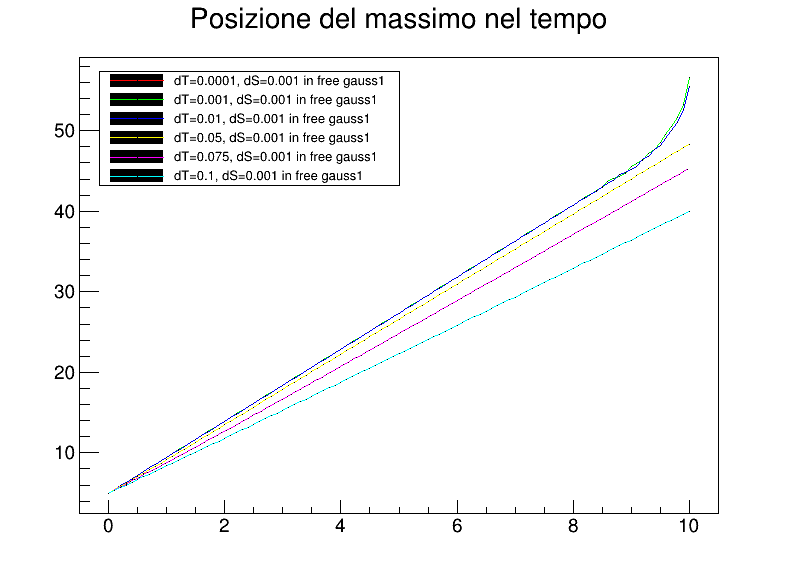
\includegraphics[width=\textwidth]{IMG/v_g1_0001}
\caption[Differenze in 0.001]{Le differenze per $dS = 0.001$}
\end{subfigure}
~
\begin{subfigure}[b]{0.49\textwidth}
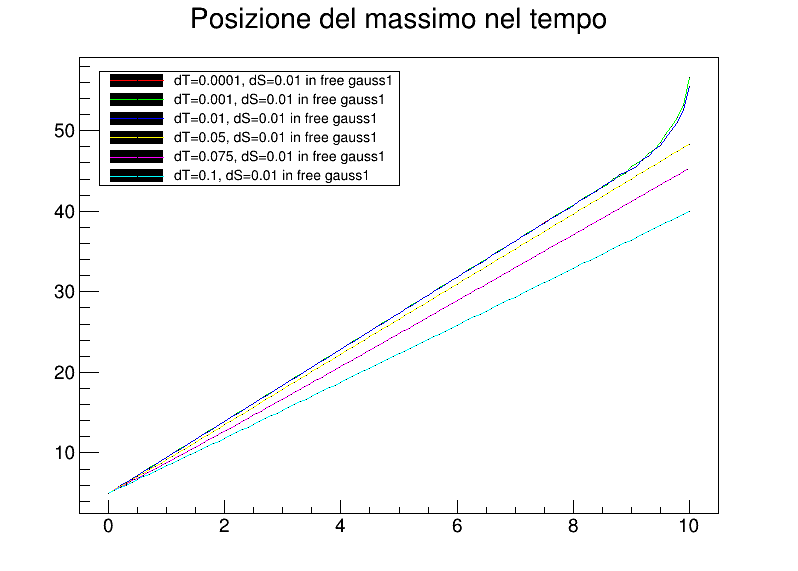
\includegraphics[width=\textwidth]{IMG/v_g1_001}
\caption[Differenze in 0.01]{Le differenze per $dS = 0.01$}
\end{subfigure}

\begin{subfigure}[b]{0.5\textwidth}
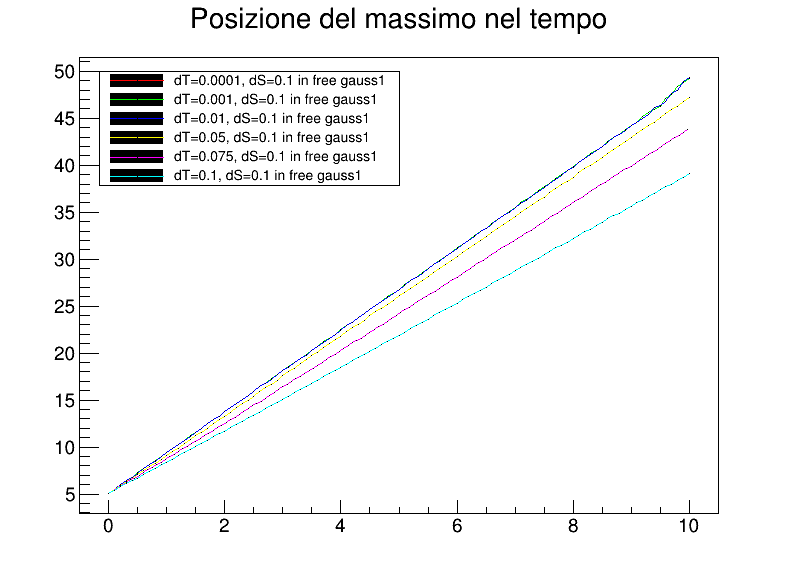
\includegraphics[width=\textwidth]{IMG/v_g1_01}
\caption[Differenze in 0.1]{Le differenze per $dS = 0.1$}
\end{subfigure}
\caption{Le posizioni dei massimi nel tempo della simulazione a vari passi temporali  e spaziali}
\end{figure}

Poi ho quindi guardato l'errore di alcune simulazioni. Scarto a priori i passi pi\`u grandi di $0.01$.

\begin{figure}
\centering
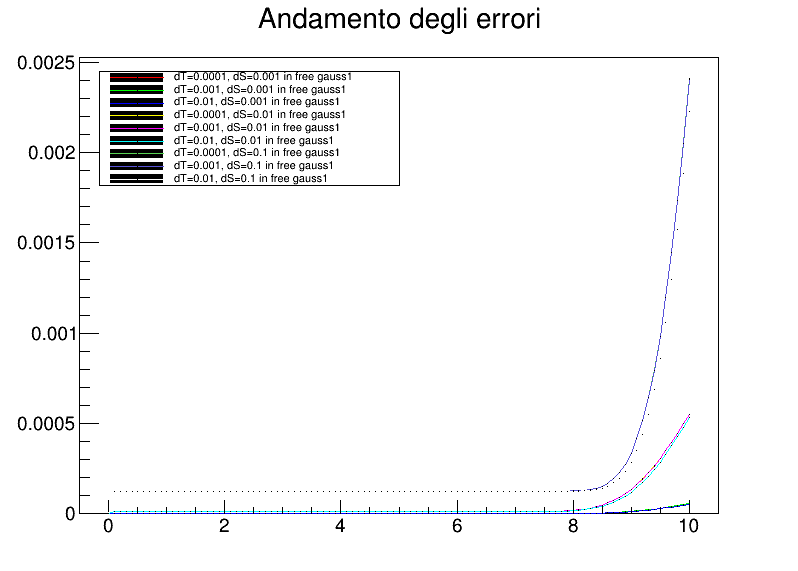
\includegraphics[width=0.7\linewidth]{IMG/e_g1full}
\caption[Errori completo]{Il grafico completo degli errori, si vede anche quanto la rilfessione cambi il modulo della funzione}
\label{fig:fullErr}
\end{figure}

A questo punto ho fatto una simulazione 

\subsection{Condizioni al contorno}
Quello che io voglio simulare \`e un pacchetto d'onda che sia partito da $-\infty$ e arrivi nel ''punto interessante'', che \`e l'area che osservo nella simulazione e poi prosegua fino all'infinito (o venga eventualmente riflesso).

Per quanto riguarda le condizioni al contorno ho avuto idee:
\begin{itemize}
	\item Non tengo conto delle condizioni al contorno, faccio in modo di usare pacchetti d'onda ristretti e blocco la simulazione quando questa va ad  avvicinarsi troppo ai bordi.
	\item Uso una forma d'onda tale per cui conosco la funzione e la sua derivata in ogni punto
	\item Emulo un ambiente chiuso (con ai lati muri di potenziale alti $\infty$)
\end{itemize}
La prima ipotesi \`e stata quella che ho usato in tutte le prove che ho effettuato prima di iniziare a raccogliere dati.

Per la seconda ipotesi dovrei usare come condizione iniziale una funzione e calcolarne la derivata per ogni passo negli estremi a priori il discorso non si applica ma i pacccheti d'onda hanno una dispersione tendono ad allargarsi, per cui se  per esempio avessi un pacchetto d'onda generico ($\Psi(x,t) = e^{ikx} \psi(x,t)$)la relazione dovrebbe essere $\partial_x \Psi(x,t) = ik \Psi(x,t) + e^{ikx}\partial_x\psi(x,t)$ e potrei quindi utilizzare le CC di Robin in caso conoscessi come la funzione si disperde nel tempo potrei ricalcolare ad ogni passo le condizioni al contorno ed applicarle. Questo per\`o mi porterebbe a svariati problemi quali l'incertezza che la simulazione e la teoria siano esattamente parallele sulla dispersione 

La terza idea equivale a utilizzare Dirichlet con il valore della funzione pari a 0 nei bordi. In pratica assomiglia alla mia prima idea, specie se blocco la simulazione prima dell'impatto

%Per cui ho deciso di ricercare un'idea che simulasse l'assenza di vincoli: ho trovato le cosiddette condizioni al contorno trasparenti.
%Ma ho lasciato perdere data la loro complessit\`a e il poco tempo a mia disposizione, in quanto utilizza la trasformazione Z
\subsection{Dispersione e forme dei pacchetti d'onda}
dispersione teoria e pratica
\subsection{Condizioni iniziali}
teoria

simulazione
\subsection{Dispersione}
teoria

pacchetti di airi non disperdono-> provare

simulazione
\subsection{Potenziali}
teoria

simulazione